% Chaptre 1

\chapter{Contexte du stage} % Main chapter title

\label{Chaptre1} % For referencing the chapter elsewhere, use \ref{Chapter1} 

Dans cette section je vais faire une présentation générale de Gigamesh, ses missions, et ses projets.

%----------------------------------------------------------------------------------------

% Define some commands to keep the formatting separated from the content 
\newcommand{\keyword}[1]{\textbf{#1}}
\newcommand{\tabhead}[1]{\textbf{#1}}
\newcommand{\code}[1]{\texttt{#1}}
\newcommand{\file}[1]{\texttt{\bfseries#1}}
\newcommand{\option}[1]{\texttt{\itshape#1}}
%----------------------------------------------------------------------------------------

\section{Présentation de Gigamesh }

Fondée en 2017 par Toufik Gozim et Mickaeel Benhassen, Gigamesh est une InsurTech française visant à se lancer dans l’assurance emprunteur. Pour ce faire, l’entreprise travaille depuis sa creéation à obtenir l’agreément deélivré par l’ACPR (Autorité de Contrôle Prudentiel et de Résolution), nécessaire pour proposer une assurance. Cette institution est chargée de surveiller les banques et assurances en France.				
\\

Gigamesh  devrait obtenir l’agrément en fin d’année 2021 et pourra donc officiellement lancer son produit d’assurance. Le choix de se positionner dans le domaine de l’assurance emprunteur n’est pas anodin. En effet, ce secteur est un oligopole détenu par des géants avec peu de place à la concurrence. Nous verrons par la suite sa complexité mais aussi l’intérêt qu’il suscite.

La loi Bourquin de février 2017, ouvre le marché de l'assurance emprunteur en permettant aux assurés de pouvoir changer leur contract d'assurance chaque année à la date anniversaire. De plus, le préavis pour effectuer ce changement est passé de 15 jours(Loi Hamon) à 2 mois. L'idée prend forme, puis le projet devient concret en octobre 2017 avec le création de la société Gigamesh SAS par Toufik Et Michael.
\\	
Gigamesh souhaite révolutionner le secteur de l’assurance emprunteur sur tous les fronts. Redonner du pouvoir d’achat, apporter une approche technologique et développer de nouvelles relations clients sont au cœur de leur vision. 



%----------------------------------------------------------------------------------------

\section{L’organigramme de Gigamesh :}
 \begin{figure}[!th]
            \centering
                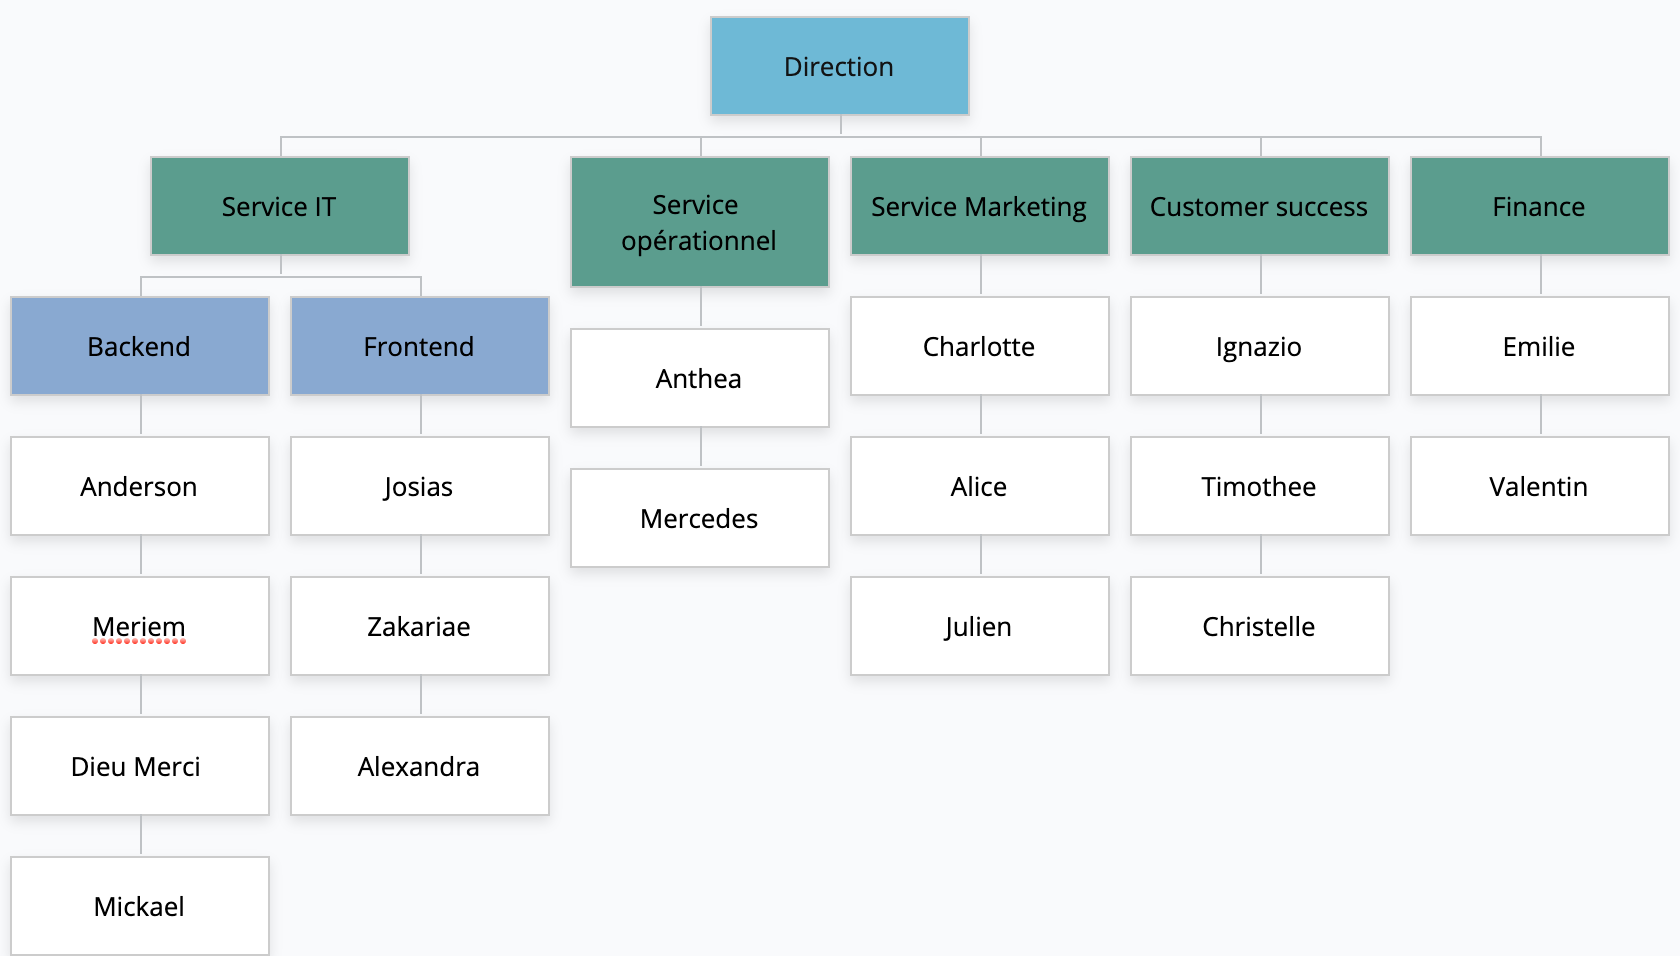
\includegraphics[width=0.8\textwidth]{Figures/orga}
	       \decoRule
		\caption[Organigramme]{Organigramme}
	\label{fig:Organigramme}
\end{figure}
 \textbf{A compléter}

\section{Localisation de Gigamesh :}

Localisé à Paris dans un espace de travail: \textbf{platform58}, \textbf{Gigamesh } profite d’un environnement de coworking et de bureaux privés. Un espace de coworking est un espace de travail partage mettant en avant l’échange et l’ouverture aux autres. Située au \textbf{58, rue de la Victoire 75009 Paris}, la \textbf{platform58} est un lieu d’innovation de la Banque Postale qui
repose sur deux briques :
\begin{itemize}
	\item Un programme d’accompagnement de startups
	\item Un lieu physique proposant la location d’espaces de travail
\end{itemize}

\section{Domaine d’activité de Gigamesh}
Nous allons voir dans cette partie le domaine dans lequel évolue \textbf{Gigamesh} et la réponse apportée pour le faire progresser.
\subsection{Assurance emprunteur}


L’assurance de prêt généralement désignée par assurance emprunteur (article L. 313-29 du code de la
consommation) est une garantie demandée par les prêteurs (les banques) lors d’une demande de prêt.
Bien que ce ne soit pas une obligation légale, elle est exigée dans la quasi-totalité des cas. Cette assurance permet de couvrir les risques de défaut de paiement quelles que soient leurs causes, ce qui explique qu’elle soit ainsi exigée. Elle comporte des garanties couvrant les risques :
\begin{itemize}
	\item D’incapacité
	\item D’invalidité
	\item Voire de perte d’emploi
\end{itemize}

\begin{figure}[!th]
\centering
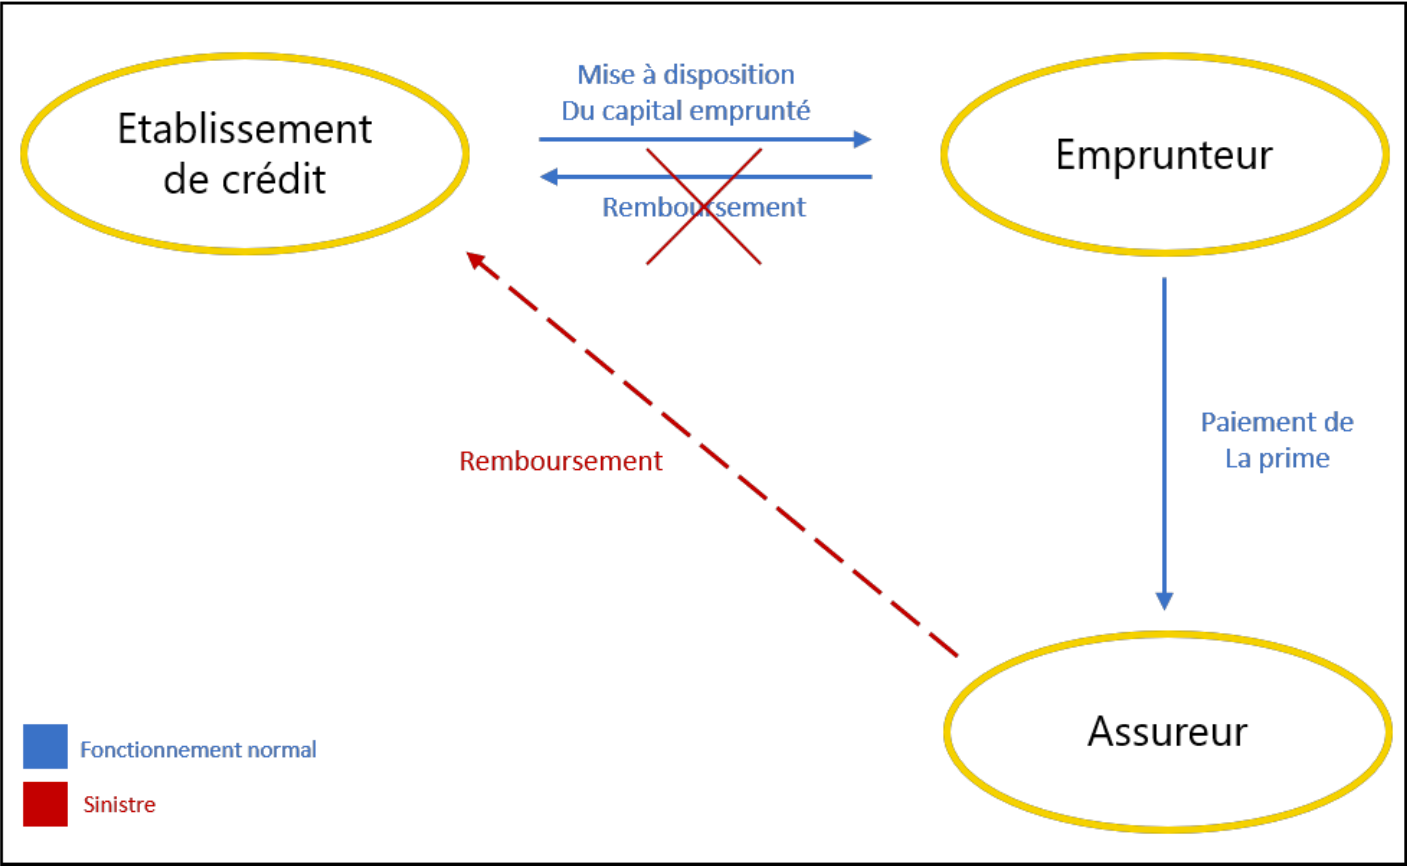
\includegraphics[width=0.8\textwidth]{Figures/emprunteur}
\decoRule
\caption[Illustration du système d'emprunt]{Illustration du système d'emprunt.}
\label{fig:Emprunt}
\end{figure}

\subsection{Assurly}
Assurly est le nom donne au produit d’assurance de Gigamesh  et represente tout le travail effectue par
l’entreprise depuis sa création. Assurly est donc le résultat du projet de Gigamesh 
Assurly est une assurance emprunteur qui bouleverse le secteur de l’assurance en créant un produit clair,
simple et au juste prix.

Tout est parti du constat que les assurances emprunteur traditionnelles ont construit leur analyse des risques sur une photographie figée de l’assuré, en décalage avec les nombreux changements que la vie réserve. Ils ont donc perdu de vue leur mission de départ : protéger en cas de problème.

Suite à 3 ans de recherche et développement, Gigamesh a réussi à associer les apports de l’innovation
technologique et leur expertise assurantielle pour créer Assurly.

Assurly est née avec l’ambition de redonner le pouvoir aux assurés en proposant un produit clair avec des
garanties all-inclusive au meilleur tarif. Assurly transforme l’assurance emprunteur grâce à une expérience client simplifiée et 100\% digitale : une souscription en moins de 10 minutes depuis son portable avec zéro paperasse, zéro rendez-vous, zéro stress !
Assurly propose de couvrir ces risques avec les garanties suivantes :

\begin{enumerate}
	\item La garantie perte totale et irréversible d’autonomie (PTIA).\\
	
Elle intervient lorsque l’assuré se trouve dans un état particulièrement grave, nécessitant le recours permanent à une tierce personne pour exercer les actes ordinaires de la vie.\\

\textbf{La couverture Assurly} : Gigamesh sera là pour vous épauler et rembourser 100\% des mensualités du reste de votre prêt. La garantie PTIA cesse au 71ème anniversaire de l’assuré.

\item La garantie incapacité temporaire totale (ITT) dénommée incapacité temporaire totale dans le contrat.\\\\

Elle intervient lorsque la personne assurée est temporairement inapte à exercer son activité professionnelle ou, si il n’en a pas, d’observer un repos complet l’obligeant à interrompre toutes ses occupations de la vie
quotidienne\\

\textbf{La couverture Assurly} : Gigamesh 
h seralà pour vous épauler et payer 100\% vos mensualités de remboursement de prêt durant votre temps d’impossibilité de travailler avec un plafond de 7500 euros par mois, quelle que soit votre perte de revenu. La garantie ITT cesse au plus tard au jour du 65ème anniversaire de l’assuré. Les affections dorsales, psychiques et psychiatriques causant l’ITT sont couvertes sans condition d’hospitalisation
ou d’intervention chirurgicale.
\begin{list}{label}{spacing}
	\item La garantie Invalidité prend deux formes :
	 \begin{enumerate}
	 	\item La garantie invalidité permanente partielle (IPP) :\\
	 	Elle intervient lorsque la personne assurée est, de façon définitive, incapable d’exercer strictement son
	 	activité après la reconnaissance de l’état d’invalidité estimé avec un taux entre 33\% et 66\%.\\
	 	
	 	\textbf{La couverture Assurly }: Gigamesh  sera là pour vous épauler et payer 50\% de l’indemnité garantie en cas d’ITT, quelle que soit votre perte de revenu, avec un plafond de 7500€ par mois. Le délai de franchise maximale est de 90 jours après l’interruption de l’activité. Les affections dorsales, psychiques et psychiatriques causant l’IPP sont couvertes sans condition d’hospitalisation
	 	ou d’intervention chirurgicale
	 	\item La garantie Invalidité Permanente Totale (I.P.T.)\\
	 	Elle intervient lorsque la personne assurée est, de
	 	façon définitive, incapable d’exercer strictement son activité professionnelle après la reconnaissance de l’état d’invalidité estimé avec un taux supérieur à 65\%\\
	 	
	 	\textbf{La couverture Assurly} : Gigamesh  sera là pour vous épauler et rembourser 100\% des mensualités du reste de votre prêt avec un plafond de 3 000 000 euros, quelle que soit votre perte de revenu. La garantie invalidité cesse au jour du 65ème anniversaire de l’assuré.
	 \end{enumerate}

\end{list}
\item La garantie décès\\
Elle intervient en cas de décès de la personne assurée. Nous serons là pour épauler votre famille et payer 100\% de vos mensualités de remboursement de votre prêt.

\end{enumerate}

\section{Objectif du stage}
Cette partie fera l’objet de la présentation du projet sur lequel j’avais travaillé et de mes propres mission dans ce celui ci:
Assurly est une plateforme digitale et innovante, qui simplifie le système d’assurance d’emprunt.
Elle est constituée des modules suivante:
\begin{itemize}
\item  Une application mobile B2C, pour la simulation de l’assurance et l’espace client,
\item  Une application B2B, pour la simulation de l’assurance et de la création d’un assure par des partenaires,
\item Un ensemble d’application de gestion, paiement en ligne et service client,
\item Une application backend pour la gestion et données et la fourniture des APIs
\end{itemize}

Les applications frontend communiquent avec le backend via une API de type Rest.
Dans le cadre de mon stage j’intervenais plus souvent dans le backend et sur les missions suivantes:

\begin{list}{•}
	\item Le déploiement et l’intégration d’un service web (Reflex) dans un environnement AWS
	\item Intégration des données en format txt dans une base de données sql dans l’environnement AWS
	\item Etude de faisabilité sur le déploiement d’une application Front-End dans un environnement AWS
	\item Sécurisation d’une API Rest développée avec la technologie Serveless d’AWS (Lambada + python).
	\item Le déploiement d’un système de web scraping dans un environnement AWS.
\end{list}
\begin{figure}[!th]
\centering
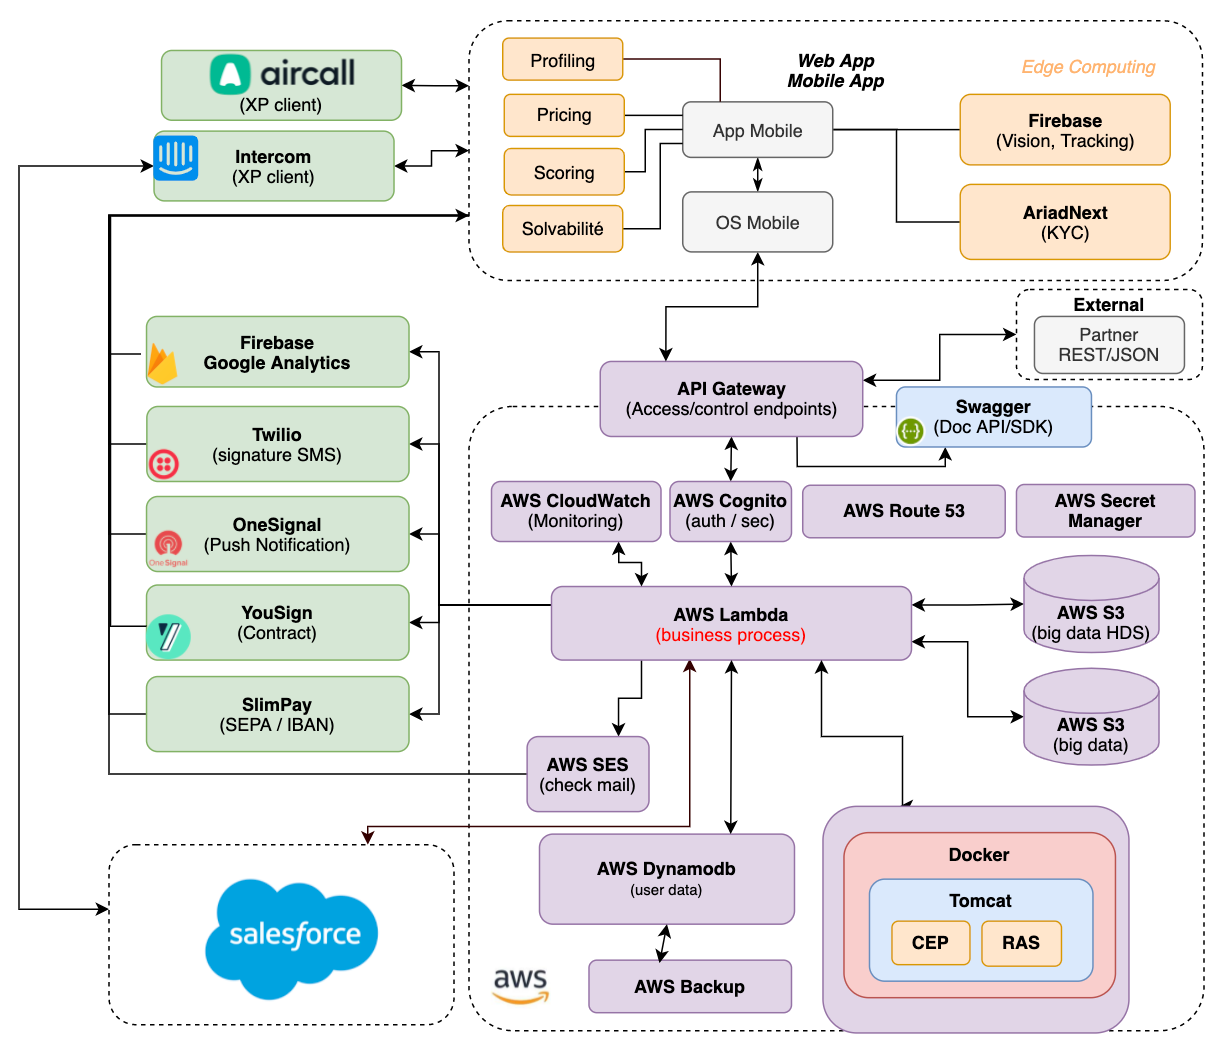
\includegraphics[width=0.8\textwidth]{Figures/architecture}
\decoRule
\caption[L'architecture]{L'architecture}
\label{fig:architecture}
\end{figure}


%----------------------------------------------------------------------------------------



